\documentclass{exercise}

\institute{Institut für Statistik und Wirtschaftsmathematik}
\title{Globalübung 5}
\author{Joshua Feld, 406718}
\course{Statistik}
\professor{Cramer}
\semester{Sommersemester 2022}
\program{CES (Bachelor)}

\begin{document}
    \maketitle


    \section*{Aufgabe 1}

    \begin{problem}
        Zur Ausrüstung von Hochschul-Instituten mit neuen Personal-Computern wurden insgesamt vier Firmen beauftragt: \(30\%\) der gelieferten Rechner stammen von Firma \(A\), jeweils \(10\%\) von den Firmen \(B\) und \(C\) und die restlichen von Firma \(D\).
        
        Bei früheren Bestellungen hat sich gezeigt, dass von den Firmen \(A\) und \(B\) jeweils \(5\%\), von Firma \(C\) \(2\%\) und von Firma \(D\) \(4\%\) der gelieferten Rechner nicht funktionstüchtig waren.
        
        Aus der letzten Lieferung wird ein Computer zufällig ausgewählt und überprüft.
        \begin{enumerate}
            \item Wie groß ist die Wahrscheinlichkeit, dass der überprüfte Rechner funktionstüchtig ist?
            \item Der überprüfte Rechner erweist sich als \emph{nicht} funktionstüchtig.
            \begin{enumerate}
                \item Mit welcher Wahrscheinlichkeit wurde der Rechner von Firma \(B\) geliefert?
                \item Welche Firma kommt am ehesten für die Lieferung des \emph{nicht} funktionstüchtigen Rechners in Frage?
            \end{enumerate}
        \end{enumerate}
    \end{problem}

    \subsection*{Lösung}
    \begin{align*}
        A: &\quad \text{``Der ausgewählte Computer stammt von Fa. }A\text{''},\\
        B: &\quad \text{``Der ausgewählte Computer stammt von Fa. }A\text{''},\\
        C: &\quad \text{``Der ausgewählte Computer stammt von Fa. }A\text{''},\\
        D: &\quad \text{``Der ausgewählte Computer stammt von Fa. }A\text{''},\\
        F: &\quad \text{``Der ausgewählte Computer ist funktionstüchtig''}.
    \end{align*}
    Weiter bezeichne \(P\) die zugehörige Wahrscheinlichkeitsverteilung.
    Dann gilt gemäß Aufgabenstellung:
    \[
        P\parentheses*{A} = 0,3, \quad P\parentheses*{B} = P\parentheses*{C} = 0,1, \quad P\parentheses*{D} = 0,5,
    \]
    \[
        P\parentheses*{F^c \mid A} = P\parentheses*{F^c \mid B} = 0,05, \quad P\parentheses*{F^c \mid C} = 0,02, \quad P\parentheses*{F^c \mid D} = 0,04.
    \]
    Hierbei werden die aus der Aufgabenstellung gegebenen (bedingten) relativen Häufigkeiten als (bedingte) Wahrscheinlichkeiten interpretiert.
    \begin{enumerate}
        \item Gemäß Aufgabenstellung bilden die Ereignisse \(A, B, C, D\) eine disjunkte Zerlegung des zugehörigen Ergebnisraums \(\Omega\).
        Daher folgt mit de Satz der totalen Wahrscheinlichkeit:
        \begin{align*}
            P\parentheses*{F^c} &= P\parentheses*{F^c \mid A}P\parentheses*{A} + P\parentheses*{F^c \mid B}P\parentheses*{B} + P\parentheses*{F^c \mid C}P\parentheses*{C} + P\parentheses*{F^c \mid D}P\parentheses*{D}\\
            &= 0,05 \cdot 0,3 + 0,05 \cdot 0,1 + 0,02 \cdot 0,1 + 0,04 \cdot 0,5 = 0,042.
        \end{align*}
        Hieraus folgt
        \[
            P\parentheses*{F} = 1 - P\parentheses*{F^c} = 0,958.
        \]
        \item 
        \begin{enumerate}
            \item Mit der Bayes-Formel folgt
            \begin{equation}\label{eq:1}
                P\parentheses*{B \mid F^c} = \frac{P\parentheses*{F^c \mid B}P\parentheses*{B}}{P\parentheses*{F^c}} = \frac{0,05 \cdot 0,1}{0,042} \approx 0,119.
            \end{equation}
            \item Analog zu (i) erhält man jeweils mit der Bayes-Formel
            \begin{align}
                P\parentheses*{A \mid F^c} &= \frac{P\parentheses*{F^c \mid A}P\parentheses*{A}}{P\parentheses*{F^c}} = \frac{0,05 \cdot 0,3}{0,042} \approx 0,357,\\
                P\parentheses*{C \mid F^c} &= \frac{P\parentheses*{F^c \mid C}P\parentheses*{C}}{P\parentheses*{F^c}} = \frac{0,02 \cdot 0,1}{0,042} \approx 0,048,\\
                P\parentheses*{D \mid F^c} &= \frac{P\parentheses*{F^c \mid D}P\parentheses*{D}}{P\parentheses*{F^c}} = \frac{0,04 \cdot 0,5}{0,042} \approx 0,476.\label{eq:4}
            \end{align}
            Gemäß \eqref{eq:1} - \eqref{eq:4} ist die bedingte Wahrscheinlichkeit, einen fehlerhaften Computer geliefert zu haben, am größten für Fa. \(D\).
            Deshalb kommt Fa. \(D\) (in diesem Sinne) am ehesten für die Lieferung in Frage.
        \end{enumerate}
    \end{enumerate}


    \section*{Aufgabe 2}

    \begin{problem}
        Gegeben seien ein Wahrscheinlichkeitsraum \(\parentheses*{\Omega, \mathfrak{U}, P}\) und drei Ereignisse \(A, B, C \in \mathfrak{U}\) mit \(P\parentheses*{B \cap C} > 0\) und \(P\parentheses*{B} < 1\).
        Betrachten Sie hierzu die folgenden Aussagen:
        \begin{enumerate}
            \item Es gilt \(P\parentheses*{A \mid B^c} + P\parentheses*{A \mid B} = 1\).
            \item Es gilt \(P\parentheses*{A^c \mid B} + P\parentheses*{A \mid B} = 1\).
            \item Es gilt \(P\parentheses*{A \cap B \mid C} = P\parentheses*{A \mid B \cap C}P\parentheses*{B \mid C}\).
            \item Falls \(P\parentheses*{C} = 1\) gilt, folgt \(P\parentheses*{A \cap C} = P\parentheses*{A}\).
            \item Aus \(P\parentheses*{C} = 1\) folgt \(C = \Omega\).
        \end{enumerate}
        Weisen sie jeweils die Gültigkeit der betreffenden Aussage nach, oder widerlegen Sie die Aussage durch Angabe eines geeigneten Gegenbeispiels.
    \end{problem}

    \subsection*{Lösung}
    Zunächst sind alle vorkommenden Wahrscheinlichkeiten wohldefiniert, denn es gilt
    \[
        P\parentheses*{B} \ge P\parentheses*{B \cap C} > 0, \quad P\parentheses*{C} \ge P\parentheses*{B \cap C} > 0, \quad P\parentheses*{B^c}= 1 - \underbrace{P\parentheses*{B}}_{< 1} > 0.
    \]
    \begin{enumerate}
        \item Falsch.
        Seien \(\Omega = \braces*{1, 2, 3}\) und \(P\) die (diskrete) Gleichverteilung auf \(\Omega\), d.h.
        \[
            P\parentheses*{E} = \frac{\absolute*{E}}{\absolute*{\Omega}}\text{ für }E \subseteq \Omega.
        \]
        Seien weiter \(A = \braces*{1}\) und \(B = \braces*{2}\).
        Dann folgt mit \(B^c = \braces*{1, 3}\)
        \[
            P\parentheses*{A \mid B^c} + P\parentheses*{A \mid B} = \frac{P\parentheses*{A \cap B^c}}{P\parentheses*{B^c}} + \frac{P\parentheses*{A \cap B}}{P\parentheses*{B}} = \frac{\absolute*{A \cap B^c}}{\absolute*{B^c}} + \frac{\absolute*{A \cap B}}{\absolute*{B}} = \frac{\absolute*{\braces*{1}}}{\absolute*{\braces*{1, 3}}} + \frac{\absolute*{\emptyset}}{\absolute*{\braces*{2}}} = \frac{1}{2} + 0 = \frac{1}{2} \ne 1.
        \]
        \item Richtig.
        Mit \(P\parentheses*{B} > 0\) gilt
        \[
            P\parentheses*{A^c \mid B} + P\parentheses*{A \mid B} = \frac{P\parentheses*{A^c \cap B}}{P\parentheses*{B}} + \frac{P\parentheses*{A \cap B}}{P\parentheses*{B}} = \frac{P\parentheses*{\parentheses*{A^c \cap B} \cup \parentheses*{A \cap B}}}{P\parentheses*{B}} = \frac{P\parentheses*{\parentheses*{A^c \cup A} \cap B}}{P\parentheses*{B}} = \frac{P\parentheses*{B}}{P\parentheses*{B}} = 1.
        \]
        \item Richtig.
        Es gilt
        \[
            P\parentheses*{A \mid B \cap C}P\parentheses*{B \mid C} = \frac{P\parentheses*{A \cap B \cap C}}{P\parentheses*{B \cap C}}\frac{P\parentheses*{B \cap C}}{P\parentheses*{C}} = \frac{P\parentheses*{A \cap B \cap C}}{P\parentheses*{C}} = P\parentheses*{A \cap B \mid C}.
        \]
        \item Richtig.
        Für \(P\parentheses*{C} = 1\) gilt zunächst
        \[
            0 \le P\parentheses*{A \cap C^c} \le P\parentheses*{C^c} = 1 - P\parentheses*{C} = 0.
        \]
        Hiermit erhält man
        \[
            P\parentheses*{A \cap C} = P\parentheses*{A \cap C} + P\parentheses*{A \cap C^c} = P\parentheses*{\parentheses*{A \cap C} \cup \parentheses*{A \cap C^c}} = P\parentheses*{A \cap \parentheses*{C \cup C^c}} = P\parentheses*{A \cap \Omega} = P\parentheses*{A}.
        \]
        \item Falsch.
        Seien \(\Omega = \braces*{1, 2}\) und \(P: \Pot\parentheses*{\Omega} \to \brackets*{0, 1}\) definiert durch
        \[
            P\parentheses*{\emptyset} = 0, \quad P\parentheses*{\braces*{1}} = 0, \quad P\parentheses*{\braces*{2}} = 1, \quad P\parentheses*{\Omega} = 1.
        \]
        Dann ist hierdurch eine Wahrscheinlichkeitsverteilung \(P\) auf \(\Pot\parentheses*{\Omega}\) definiert, die den Kolmogorov-Axiomen genügt, aber für \(C = \braces*{2}\) gilt
        \[
            C = \braces*{2} \ne \braces*{1, 2} = \Omega \quad \text{und} \quad P\parentheses*{C} = P\parentheses*{\braces*{2}} = 1.
        \]
    \end{enumerate}


    \section*{Aufgabe 3}

    \begin{problem}
        Eine Firma möchte zur Sicherung ihres Produktionsgeländes eine Alarmanlage installieren lassen, die aus einem Sensor und einer Sirene bestehen sol.
        Die zuständige Technikerin rät, jeweils zwei Sensoren und zwei Sirenen einzubauen, da diese Komponenten nicht hundertprozentig ausfallsicher sind.
        Sie schlägt folgende beiden Konfigurationen vor:
        \begin{center}
            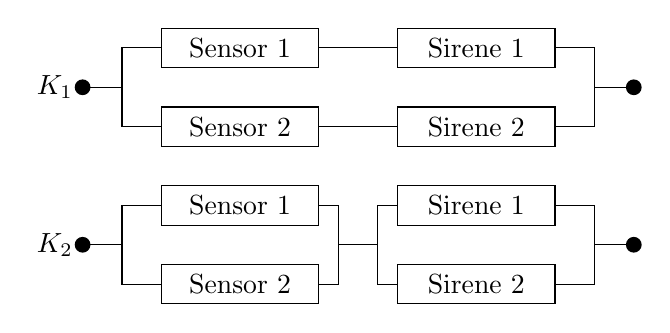
\begin{tikzpicture}
                \fill (0,0) circle (1mm);
                \node[anchor=east] at (0,0) {\(K_1\)};
                \fill (7,0) circle (1mm);
                \draw (1,.25) rectangle (3,.75) node[pos=.5] {Sensor \(1\)};
                \draw (1,-.25) rectangle (3,-.75) node[pos=.5] {Sensor \(2\)};
                \draw (4,.25) rectangle (6,.75) node[pos=.5] {Sirene \(1\)};
                \draw (4,-.25) rectangle (6,-.75) node[pos=.5] {Sirene \(2\)};
                \draw (0,0) -- (.5,0);
                \draw (1,.5) -- (.5,.5) -- (.5,-.5) -- (1,-.5);
                \draw (6.5,0) -- (7,0);
                \draw (6,.5) -- (6.5,.5) -- (6.5,-.5) -- (6,-.5);
                \draw (3,.5) -- (4,.5);
                \draw (3,-.5) -- (4,-.5);
                \begin{scope}[shift={(0,-2)}]
                    \fill (0,0) circle (1mm);
                    \node[anchor=east] at (0,0) {\(K_2\)};
                    \fill (7,0) circle (1mm);
                    \draw (1,.25) rectangle (3,.75) node[pos=.5] {Sensor \(1\)};
                    \draw (1,-.25) rectangle (3,-.75) node[pos=.5] {Sensor \(2\)};
                    \draw (4,.25) rectangle (6,.75) node[pos=.5] {Sirene \(1\)};
                    \draw (4,-.25) rectangle (6,-.75) node[pos=.5] {Sirene \(2\)};
                    \draw (0,0) -- (.5,0);
                    \draw (1,.5) -- (.5,.5) -- (.5,-.5) -- (1,-.5);
                    \draw (6.5,0) -- (7,0);
                    \draw (6,.5) -- (6.5,.5) -- (6.5,-.5) -- (6,-.5);
                    \draw (3,.5) -- (3.25,.5) -- (3.25,-.5) -- (3,-.5);
                    \draw (3.25,0) -- (3.75,0);
                    \draw (4,.5) -- (3.75,.5) -- (3.75,-.5) -- (4,-.5);
                \end{scope}
            \end{tikzpicture}
        \end{center}
        Die Konfigurationen \(K_1\) bzw. \(K_2\) sind funktionstüchtig, wenn zwischen den betreffenden Knotenpunkten eine Verbindung aus intakten Komponenten besteht.
        
        Es sei vorausgesetzt, dass die vier Komponenten in jeder Konfiguration unabhängig voneinander ausfallen.
        Die Ausfallwahrscheinlichkeit für die Sensoren betrage jeweils \(q_1 \in \parentheses*{0, 1}\) und die Ausfallwahrscheinlichkeit für die Sirenen jeweils \(q_2 \in \parentheses*{0, 1}\) (für den Ausfall innerhalb eines festen Zeitraums).
        \begin{enumerate}
            \item Welche der beiden Konfigurationen \(K_1, K_2\) besitzt eine höhere Zuverlässigkeit, d.h. eine höhere Intaktwahrscheinlichkeit?
            Gilt dies für alle Werte \(q_1, q_2 \in \parentheses*{0, 1}\)?
            \item Berechnen Sie zu beiden Konfigurationen \(K_1, K_2\) jeweils die Intaktwahrscheinlichkeiten für \(q_1 = 0,2\) und \(q_2 = 0,1\).
        \end{enumerate}
    \end{problem}

    \subsection*{Lösung}
    Es bezeichne
    \begin{align*}
        A_j&: \quad \text{``Sensor }j\text{ intakt''},\\
        B_j&: \quad \text{``Sirene }j\text{ intakt''},\\
        I_j&: \quad \text{``Konfiguration }j\text{ intakt''}
    \end{align*}
    für \(j \in \braces*{1, 2}\).
    Weiter bezeichne \(P\) die zugehörige Wahrscheinlichkeitsverteilung.
    Dann gilt gemäß Aufgabenstellung mit \(p_1 = 1 - q_1\) und \(p_2 = 1 - q_2\):
    \[
        P\parentheses*{A_j} = 1 - q_1 = p_1, \quad P\parentheses*{B_j} = 1 - q_2 = p_2, \quad j \in \braces*{1, 2}.
    \]
    \begin{enumerate}
        \item Mit den gewählten Bezeichnungen gilt
        \begin{align*}
            P\parentheses*{I_1} &= P\parentheses*{\parentheses*{A_1 \cap B_1} \cup \parentheses*{A_2 \cap B_2}}\\
            &= P\parentheses*{A_1 \cap B_1} + P\parentheses*{A_2 \cap B_2} - P\parentheses*{A_1 \cap B_1 \cap A_2 \cap B_2}\\
            &= P\parentheses*{A_1}P\parentheses*{B_1} + P\parentheses*{A_2}P\parentheses*{B_2} - P\parentheses*{A_1}P\parentheses*{B_1}P\parentheses*{A_2}P\parentheses*{B_2}\\
            &= p_1 p_2 + p_1 p_2 - p_1^2 p_2^2\\
            &= p_1 p_2\parentheses*{2 - p_1 p_2}.
        \end{align*}
        Hierbei ging im dritten Schritt ein, dass die Ereignisse \(A_1, A_2, B_1, B_2\) gemäß Voraussetzung (gemeinsam) stochastisch unabhängig sind.
        Damit sind auch die Ereignisse \(A_1 \cup A_2\) und \(B_1 \cup B_2\) stochastisch unabhängig.
        Es gilt also
        \[
            P\parentheses*{\parentheses*{A_1 \cup A_2} \cap \parentheses*{B_1 \cup B_2}} = P\parentheses*{A_1 \cup A_2}P\parentheses*{B_1 \cup B_2}.
        \]
        Hiermit folgt
        \begin{align*}
            P\parentheses*{I_2} &= P\parentheses*{\parentheses*{A_1 \cup A_2} \cap \parentheses*{B_1 \cup B_2}}\\
            &= P\parentheses*{A_1 \cup A_2}P\parentheses*{B_1 \cup B_2}\\
            &= \parentheses*{P\parentheses*{A_1} + P\parentheses*{A_2} - P\parentheses*{A_1 \cap A_2}}\parentheses*{P\parentheses*{B_1} + P\parentheses*{B_2} - P\parentheses*{B_1 \cap B_2}}\\
            &= \parentheses*{P\parentheses*{A_1} + P\parentheses*{A_2} - P\parentheses*{A_1}P\parentheses*{A_2}}\parentheses*{P\parentheses*{B_1} + P\parentheses*{B_2} - P\parentheses*{B_1}P\parentheses*{B_2}}\\
            &= \parentheses*{2p_1 - p_1^2}\parentheses*{2p_2 - p_2^2}\\
            &= p_1 p_2\parentheses*{2 - p_1}\parentheses*{2 - p_2}.
        \end{align*}
        Insgesamt erhält man schließlich
        \begin{align*}
            P\parentheses*{I_2} - P\parentheses*{I_1} &= p_1 p_2\parentheses*{2 - p_1}\parentheses*{2 - p_2} - p_1 p_2\parentheses*{2 - p_1 p_2}\\
            &= p_1 p_2\parentheses*{4 - 2p_1 - 2p_2 + p_1 p_2 - 2 + p_1 p_2}\\
            &= 2p_1 p_2\parentheses*{1 - p_1 - p_2 + p_1 p_2}\\
            &= 2p_1 p_2\parentheses*{1 - p_1}\parentheses*{1 - p_2}\\
            &= 2\parentheses*{1 - q_1}\parentheses*{1 - q_2}q_1 q_2 > 0
        \end{align*}
        für alle \(q_1, q_2 \in \parentheses*{0, 1}\).
        Somit besitzt die Konfiguration \(K_2\) für sämtliche Werte \(q_1, q_2 \in \parentheses*{0, 1}\) die höhere Intaktwahrscheinlichkeit und damit (in diesem Sinne) die höhere Zuverlässigkeit.
        \item Für \(q_1 = 0,2\) und \(q_2 = 0,1\) sind \(p_1 = 1 - q_1 = 0,8\) und \(p_2 = 1 - q_2 = 0,9\).
        Es folgt
        \begin{align*}
            P\parentheses*{I_1} &= p_1 p_2\parentheses*{2 - p_1 p_2} = 0,8 \cdot 0,9 \cdot \parentheses*{2 - 0,8 \cdot 0,9} = 0,9216,\\
            P\parentheses*{I_2} &= p_1 p_2\parentheses*{2 - p_1}\parentheses*{2 - p_2} = 0,8 \cdot 0,9 \cdot \parentheses*{2 - 0,8} \cdot \parentheses*{2 - 0,9} = 0,9504.
        \end{align*}
    \end{enumerate}
\end{document}
